

\section{Experiment motivation}
The introduction lists several questions that this report should contribute to.
One of the questions concerns how collective decision making influences the emergence of self-assembly.
Swarm behaviour found in nature displays how simple agents collectively can make a decision.
The goal of this experiment is therefore to design a similar environment to promote this form of collective behaviour.
In this environment the robots have to form swarms for survival, and collectively decide if they should self-assemble or attempt an escape.

The experiment also allows investigation into the other questions this report contributes to.
By varying the parameters of the experiment it is possible to observe how different docking mechanisms and assembly protocols influence the self-assembly behaviour of the robots.
Section \ref{sec:results} further describes how this experiment can answer these questions.
\section{Experiment setup}
\label{sec:description}
For this experiment a micro-organism environment is imagined, where the organisms find themselves in some liquid pool. 
The micro-organisms are the agents in our system and are represented as swarm bots.
The main functions of the robots are, in addition to movement, foraging and self-assembly.

The robots find themselves in a pond.
In the pond there are nutrients which the robots can feed on to replenish their energy.
At the same time the pond also contains larger predator organisms which wants to feed on the robots.
It is imagined that the robots can assemble to form larger structures.
The robots can protect themselves from the predator organisms by forming a larger structure which the predator is unable to eat.
When the robots are assembled they may eat the larger predator to replenish energy as well.
The predators come in multiple sizes, and to gain an advantage the robots must form a large enough structure.
Maintaining the assembled structure cost energy, and the robots therefore have an incentive to disassemble once the structure is no longer required.

\section{Environment}
The imagined pond environment can be represented as a rectangular box(figure \ref{fig:environment}), containing the robots, nutrients and predators.
Initially the environment is populated with nutrients, robots, and predators placed at random positions in the environment.
When a nutrient is consumed, a new one is placed at a random position in the environment.
Additionally, to ensure fairness the predators cannot be placed within a threshold radius of a robot. 

\begin{figure}[H]
	
	\centering
	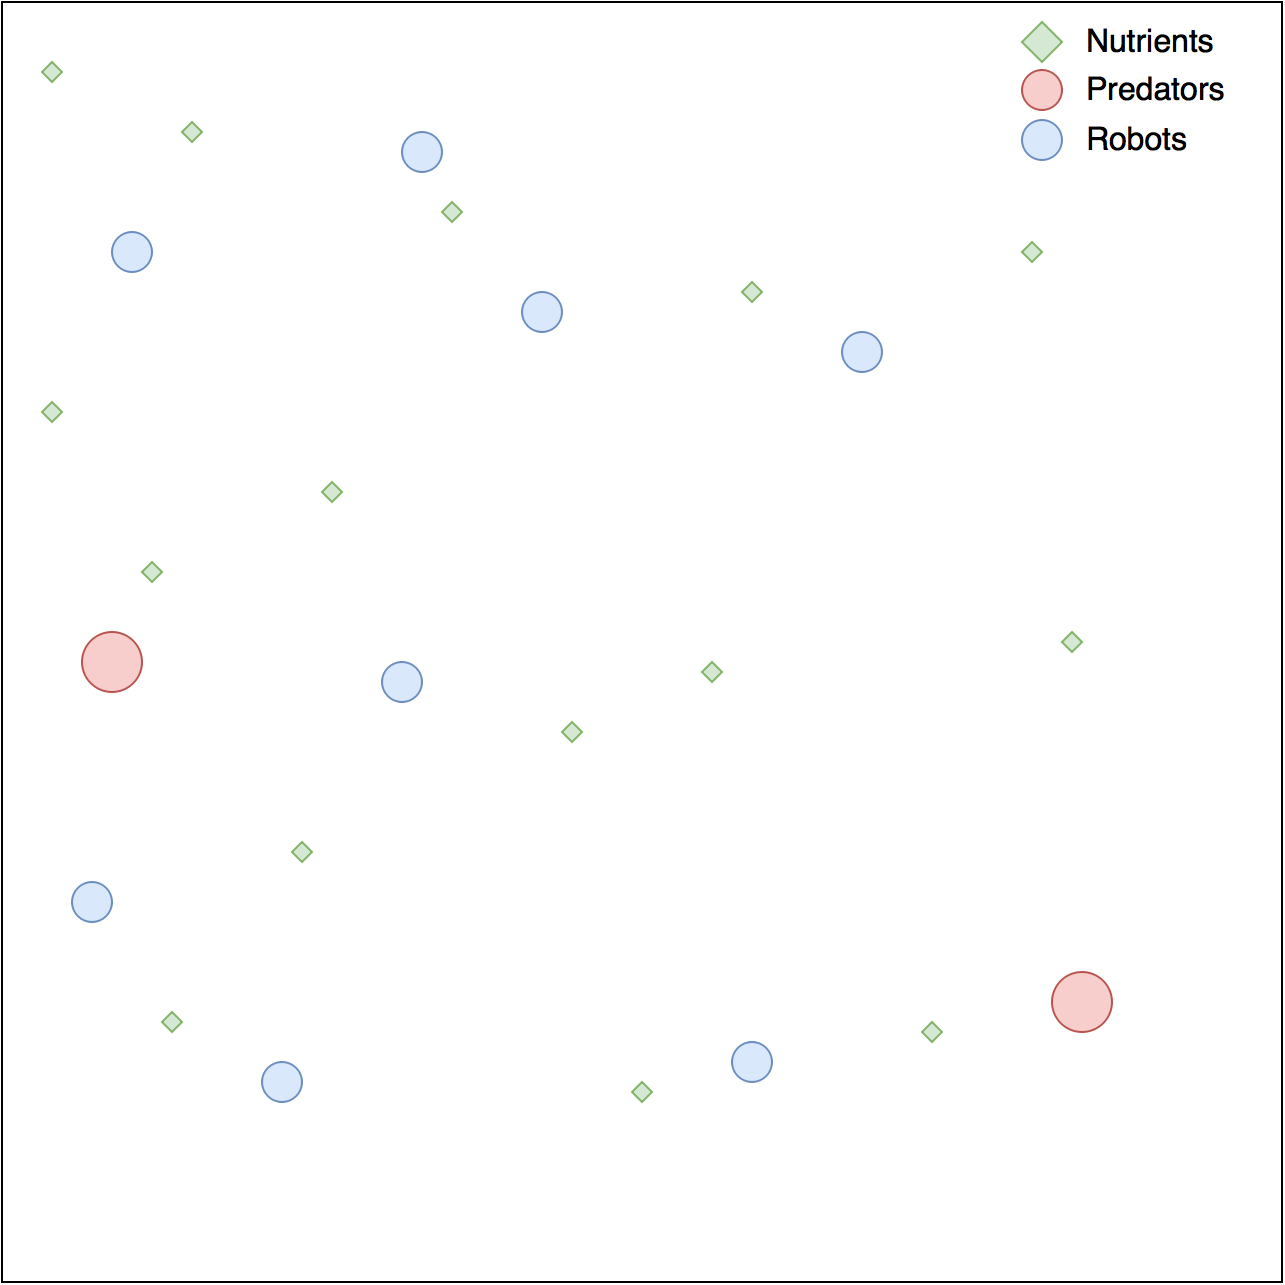
\includegraphics[width=0.65\textwidth]{chapters/res/Environment.png}
	\caption{Initial configuration of the environment.}
	\label{fig:environment}
\end{figure}

\section{Roborobo overview}
	\subsection{Agent observers}
	\subsection{Agent controllers}
	\subsection{World observers}














\section{Roborobo modifications}
	\subsection{Robot Groups}
	As mentioned in the description, roborobo does not support self-assembly out of the box.
	Self-assembly support therefore requires adding additional abstractions to roborobo.
	The high level abstraction that encapsulates the behavior for connected robots is called a \emph{Robot group}.
	All robots that are capable of self-assembly are robot groups.
	This means that single robots that are not connected are simply robot groups with one member.
	The responsibilities of the robot group is to take care of group movement, handling collisions, connecting and disconnecting. 
	\subsubsection{Movement}
	In the roborobo framework the robots movement is decided by the robot controller by requesting a certain angular and translational velocity.
	The movement of a group is decided by first converting the desired direction and velocity into a translation vector.
	\begin{figure}[H]
		\centering
		$v_x = translation \cdot \cos(angle)$ \\
		$v_y = translation \cdot sin(angle)$
	\end{figure}
	The combined movement for the group is then decided by averaging the translation vectors from each member in the group.
	\begin{figure}[H]
		\centering
		$v_t = \frac{1}{n}\sum_{i=0}^{n} v_{i}$
	\end{figure}
	Once the translation vector for the group is computed it can be applied to each member of the group by converting it back to the format of direction and velocity that roborobo uses.
	
	\subsubsection{Collisions}
	Roborobo already performs collision detection for robots, but in robot groups some additional logic is required.
	The collision behavior for robots is that if they collide with a solid object, they stop.
	This is a problem for groups of more than one robot because if one robot collides it may get left behind by the rest of the group.
	This is solved by backing up the position of each robot in a group before applying the computed translation.
	If a robot in the group collides with something, the robots in the group are reverted to their original position.
	\subsubsection{Connections}
	It is useful to treat the connections between robots in a group as a graph, where the robots are nodes and connections are edges.
	Connecting robots can then be treated as simply adding an edge between the two nodes representing that are connecting.
	In the same way, disconnecting then consists of removing the edge between the nodes representing the connected robots.
	In the case that a robot has multiple connections in the group extra care has to be taken, because removing one edge may split the graph into two smaller sub-graphs.
	If this occurs the two sub-graphs must now be treated as two new separate groups.
	It can be determined if a robot can simply be disconnected, or if we have to split the group by finding out if there is a cycle that leads back to the robot that is to be disconnected.
	The existence of a cycle is determined by first removing the edge representing the connection, and then performing a depth first search.
	
	 
	\subsection{Docking mechanism}
	As described in section \ref{sec:mechanisms}, there is a wide variety of docking mechanisms.
	The docking mechanism implemented is therefore highly configurable, to suppo
		
		\subsubsection{Connection validation}
	\subsection{Local communication}
		\subsubsection{Message aggregation, message lattice}
		
		
	\subsection{Predators}
		\subsubsection{Search strategy}
		\subsubsection{Hunting strategy}
	\subsection{Energy drain}
		\subsubsection{Passive}
		\subsubsection{Active}

\section{CTRNN}
	\subsection{Drain}
	\subsection{Activation function}
	\subsection{Topologies}
		\subsubsection{Dense}
		\subsubsection{Sparse}

\section{Evolutionary algorithm}
	\subsection{Genotype}
	\subsection{Initialization}
	\subsection{Mutation operators}
		\subsubsection{Random}
		\subsubsection{Incremental}
	\subsection{Selection mechanism}

\section{Data gathering}
	\section{Loggers}
	\section{Analysis}
	
\subsection{Extras/Appendix?}
	\subsection{Parallelization}
	\subsection{Python graph tool}
	\subsection{System configuration}
	
	